%Generazione delle variabili che andranno a sostituire quelle del template `HomePage.tex`
\newcommand{\documento}{Manuale Utente}
\newcommand{\nomedocumentofisico}{ManualeUtente\_v2\_0\_0.pdf}
\newcommand{\redazione}{\SM, \\ & \GN}
\newcommand{\verifica}{\MV, \\ & \MP}
\newcommand{\approvazione}{\GR, \\ & \SM}
\newcommand{\uso}{Esterno}
\newcommand{\destinateTo}{\TV, \\ & \RC, \\ & \ZU}
\newcommand{\datacreazione}{13 Maggio 2016}
\newcommand{\datamodifica}{04 Giugno 2016}
\newcommand{\stato}{Approvato}
\newcommand{\versione}{2}

\def\TABELLE{false}	%abilita - disabilita l'indice delle tabelle
\def\FIGURE{false} 	%abilita - disabilita l'indice delle figure

%Layout del documento 
\documentclass[a4paper,11pt]{article}

%***IMPORTAZIONE PACKAGE***
\usepackage{ifthen}
\usepackage[italian]{babel}
\usepackage[utf8]{inputenc}
\usepackage[T1]{fontenc}
\usepackage{float}
\usepackage{chapterbib}
\usepackage{graphicx}
\usepackage[a4paper,top=2.5cm,bottom=2.5cm,left=2.5cm,right=2.5cm]{geometry}
\usepackage[colorlinks=true, urlcolor=black, citecolor=black, linkcolor=black]{hyperref}
\usepackage{booktabs}
\usepackage{fancyhdr}
\usepackage{totpages}
\usepackage{tabularx, array}
\usepackage{dcolumn}
\usepackage{epstopdf}
\usepackage{booktabs}
\usepackage{fancyhdr}
\usepackage{longtable}
\usepackage{calc}
\usepackage{datatool}
\usepackage[bottom]{footmisc}
\usepackage{listings} 
\usepackage{textcomp}
\usepackage{titlesec}
\usepackage{rotating} 
\usepackage{multirow}
\usepackage{placeins}
\usepackage{color}
\usepackage[table,usenames,dvipsnames]{xcolor}
\usepackage{hyperref}
\usepackage{makecell}
\usepackage{hyperref}


%***STILE PAGINA***
\pagestyle{fancy}
%no indentazione paragrafo
\setlength{\parindent}{0pt}

%***INTESTAZIONE***
\lhead{\Large{\progetto} \\ \footnotesize{\documento}}
\rhead{
\includegraphics[keepaspectratio = true, width = 25px] {../../Template/icone/LogoGruppo.png}}
\renewcommand{\headrulewidth}{0.4pt}  %Linea sotto l'intestazione

%***PIÈ DI PAGINA***
\lfoot{\textit{\gruppoLink}\\ \footnotesize{\email}}
\rfoot{\thepage} %per le prime pagine: mostra solo il numero romano
\cfoot{}
\renewcommand{\footrulewidth}{0.4pt}   %Linea sopra il piè di pagina

%***INSERIMENTO DI NUOVE SOTTOSEZIONI
\setcounter{secnumdepth}{7}		% mostra nel documento fino al livello 8 (1.2.3.4.5.6.7.8)
\setcounter{tocdepth}{7}			% mostra nell'indice fino al livello 8 (1.2.3.4.5.6.7.8)

%***LA SOTTOSEZIONE PARAGRAPH VIENE VISUALIZZATA COME UNA SECTION
\titleformat{\paragraph}{\normalfont\normalsize\bfseries}{\theparagraph}{1em}{}
\titlespacing*{\paragraph}{0pt}{3.25ex plus 1ex minus .2ex}{1.5ex plus .2ex}

\titleformat{\subparagraph}{\normalfont\normalsize\bfseries}{\thesubparagraph}{1em}{}
\titlespacing*{\subparagraph}{0pt}{3.25ex plus 1ex minus .2ex}{1.5ex plus .2ex}

\makeatletter
\newcounter{subsubparagraph}[subparagraph]
\renewcommand\thesubsubparagraph{%
  \thesubparagraph.\@arabic\c@subsubparagraph}
\newcommand\subsubparagraph{%
  \@startsection{subsubparagraph}    % counter
    {6}                              % level
    {\parindent}                     % indent
    {3.25ex \@plus 1ex \@minus .2ex} % beforeskip
    {0.75em}                           % afterskip
    {\normalfont\normalsize\bfseries}}
\newcommand\l@subsubparagraph{\@dottedtocline{6}{10em}{5.5em}} %gestione dell'indice
\newcommand{\subsubparagraphmark}[1]{}
\makeatother

\makeatletter
\newcounter{subsubsubparagraph}[subsubparagraph]
\renewcommand\thesubsubsubparagraph{%
  \thesubsubparagraph.\@arabic\c@subsubsubparagraph}
\newcommand\subsubsubparagraph{%
  \@startsection{subsubsubparagraph}    % counter
    {7}                              % level
    {\parindent}                     % indent
    {3.25ex \@plus 1ex \@minus .2ex} % beforeskip
    {0.75em}                           % afterskip
    {\normalfont\normalsize\bfseries}}
\newcommand\l@subsubsubparagraph{\@dottedtocline{7}{10em}{6.5em}} %gestione dell'indice
\newcommand{\subsubsubparagraphmark}[1]{}
\makeatother


%Comandi generali
%Generali
\newcommand{\progetto}{QuizziPedia}
\newcommand{\gruppo}{TheFellowshipOfTheCode}
\newcommand{\gruppoLink}{\href{http://thefellowshipofthecode.github.io/}{TheFellowshipOfTheCode}}
\newcommand{\email}{\href{mailto:thefellowshipofthecode@gmail.com}{thefellowshipofthecode@gmail.com}}

%Documenti
\newcommand{\AdR}{Analisi dei Requisiti}
\newcommand{\NdP}{Norme di Progetto}
\newcommand{\PdP}{Piano di Progetto}
\newcommand{\SdF}{Studio di Fattibilità}
\newcommand{\PdQ}{Piano di Qualifica}
\newcommand{\VI}{Verbale Interno}
\newcommand{\VE}{Verbale Esterno}
\newcommand{\ST}{Specifica Tecnica}
\newcommand{\DDP}{Definizione di Prodotto}
\newcommand{\MU}{Manuale Utente}
\newcommand{\G}{Glossario}
\newcommand{\LdP}{Lettera di Presentazione}
\newcommand{\NdPv}{NormeDiProgetto\_v\_1\_0\_0}
\newcommand{\PdPv}{PianoDiProgetto\_v\_1\_0\_0}
\newcommand{\PdQv}{PianoDiQualifica\_v\_1\_0\_0}
\newcommand{\SdFv}{StudioDiFattibilità\_v\_1\_0\_0}

%Componenti del gruppo
\newcommand{\AF}{Alberto Ferrara}
\newcommand{\SM}{Simone Magagna}
\newcommand{\FB}{Franco Berton}
\newcommand{\MP}{Marco Prelaz}
\newcommand{\MV}{Mattia Varotto}
\newcommand{\GN}{Matteo Gnoato}
\newcommand{\GR}{Matteo Granzotto}

%Ruoli
\newcommand{\RdP}{Responsabile di Progetto}
\newcommand{\Res}{Responsabile}
\newcommand{\Amm}{Amministratore}
\newcommand{\Ver}{Verificatore}
\newcommand{\Prog}{Progettista}
\newcommand{\Progr}{Programmatore}
\newcommand{\Ana}{Analista}
\newcommand{\RdPs}{Responsabili di Progetto}
\newcommand{\Ress}{Responsabile}
\newcommand{\Amms}{Amministratori}
\newcommand{\Vers}{Verificatori}
\newcommand{\Progs}{Progettisti}
\newcommand{\Progrs}{Programmatori}
\newcommand{\Anas}{Analisti}

%Professori e proponente
\newcommand{\TV}{Prof. Tullio Vardanega}
\newcommand{\RC}{Prof. Riccardo Cardin}
\newcommand{\ZU}{Zucchetti S.P.A.}
\newcommand{\proponente}{Zucchetti S.P.A.}

\newcommand{\diaryEntry}[5]{#2 & \emph{#4} & #3 & #5 & #1\\ \hline}

%comando per una nuova riga nella tabella del diario delle modifiche
\newcommand{\specialcell}[2][c]{%
	\begin{tabular}[#1]{@{}c@{}}#2\end{tabular}}

\renewcommand*\sectionmark[1]{\markboth{#1}{}}
\renewcommand*\subsectionmark[1]{\markright{#1}}

%Pediodi di lavoro 
\newcommand{\AR}{Analisi dei Requisiti}
\newcommand{\AD}{Analisi dei Requisiti in Dettaglio}
\newcommand{\PA}{Progettazione Architetturale}
\newcommand{\PD}{Progettazione di Dettaglio}
\newcommand{\CO}{Codifica}
\newcommand{\VV}{Verifica e Validazione}

% Revisioni
\newcommand{\RR}{Revisione dei Requisiti}
\newcommand{\RP}{Revisione di Progettazione}
\newcommand{\RQ}{Revisione di Qualifica}
\newcommand{\RA}{Revisione di Accettazione}

% Comandi analisi dei requisiti
\newcommand{\uau}{utente autenticato}
\newcommand{\uaus}{utenti autenticati}
\newcommand{\uaupro}{utente autenticato pro}
\newcommand{\uauspro}{utenti autenticati pro}

\newcommand{\myincludegraphics}[2][]{%
	\setbox0=\hbox{\phantom{X}}%
	\vtop{
		\hbox{\phantom{X}}
		\vskip-\ht0
		\hbox{\includegraphics[#1]{#2}}}}

\begin{document}
	
%inclusione template HomePage
\begin{center}

%
\includegraphics[width=1em]{../../../Template/icone/LogoGruppo.png}
\begin{large} \textbf{\gruppoLink} \end{large}
%
\includegraphics[width=1em]{../../../Template/icone/LogoGruppo.png}
\vspace{0.2em}

\hrule
\vspace{3em}


\includegraphics[keepaspectratio = true, width=8cm]{../../../Template/icone/LogoGruppo.png}

%Prima pagina senza intestazione né piè di pagina	
\thispagestyle{empty}

%Le informazioni del documento sono ancorate a fine pagina
\vfill

%Copertina
\begin{center} 
  \begin{Huge}
  {\fontsize{15mm}{20mm}\selectfont \progetto} 
  \end{Huge}
\end{center}

\begin{Huge} \documento \end{Huge}

\begin{center}
\textbf{Informazioni sul documento} \\ \vspace{2em}
\small
\begin{tabular}{r|l}
	\textbf{Nome Documento} & \nomedocumentofisico \\
	\textbf{Versione}	& 1\\
	\textbf{Data di Creazione} & \datacreazione\\
	\textbf{Data ultima modifica} & \datamodifica\\
	\textbf{Stato} & \stato \\
	\textbf{Redazione}	& \redazione\\
	\textbf{Verifica}	& \verifica\\
	\textbf{Approvazione}	& \approvazione\\
	\textbf{Uso}  & \uso\\
	\textbf{Distribuzione} & \gruppo \\
	\textbf{Destinato a}  &  \destinateTo \\
	\textbf{Email di riferimento} & \email
\end{tabular}
\end{center}

\normalsize
%Sommario
\textbf{Sommario\\} 
Documento contenente le norme di progetto che il gruppo \textit{\gruppo} seguirà durante tutte le fasi di realizzazione del prodotto \textit{\progetto}.

%\vfill %cosa fa?
\end{center}
\clearpage


%Registro delle modifiche e indice 
%si usa la numerazione romana per gli indici e la tabella delle modifiche
\pagenumbering{Roman}
\newcommand{\modificheuno} 
{	
	0.0.3 & Inseriti i primi riferimenti informativi & \specialcell[t]{\GN \\ \prog} & 2016-02-26
	\\\midrule
	0.0.2 & Stesura scopo del documento, scopo del prodotto , riferimenti normativi & \specialcell[t]{\GN \\ \prog} & 2016-02-26
	\\\midrule
	0.0.1 & Creato template documento & \specialcell[t]{\GN \\ \prog} & 2016-02-26
	\\\midrule
}
\newcommand{\modifichedue}
{
}
\newpage
%Inserisce il link all'indice
%\addcontentsline{toc}{section}{Indice}
\tableofcontents
\clearpage 

%Se è stata impostata a true la variabile per la lista delle tabelle, la mostra
\ifthenelse{\equal{\TABELLE}{true}} 
{\listoftables \newpage}{}

%Se è stata impostata a true la variabile per la lista delle figure, la mostra
\ifthenelse{\equal{\FIGURE}{true}}
{\listoffigures \newpage}{}

%Da qui comincia la numerazione normale
\pagenumbering{arabic}

%Imposta il formato di visualizzazione
\rfoot{\thepage~di~\pageref{TotPages}}
\newpage
\listoffigures

\newpage
%sezioni documento
\newpage
\section{Introduzione}

\subsection{Scopo del documento}
Il presente documento ha lo scopo di definire in dettaglio la struttura e il funzionamento delle componenti del progetto \progetto. Questo documento servirà come guida per i \textit{\Progrs} del gruppo \gruppo fornendo direttive e vincoli per la realizzazione del \textit{progetto\ped{G}}.

\subsection{Scopo del prodotto}
Lo scopo del prodotto è di permettere la creazione e gestione di questionari in grado di identificare le lacune dei candidati prima, durante e al termine di un corso di formazione. 
\\Il sistema dovrà offrire le seguenti funzionalità:
\begin{itemize}
	\item
	Archiviare questionari in un server suddivisi per argomento;
	\item
	Somministrare all'utente, tramite un'interfaccia, questionari specifici per argomento scelto;
	\item
	Verificare e valutare i questionari scelti dagli utenti in base alle risposte date.
\end{itemize}
La parte destinata ai creatori di questionari dovrà essere fruibile attraverso un \textit{browser\ped{G}} desktop, abilitato all'utilizzo delle tecnologie \textit{HTML5\ped{G}}, \textit{CSS3\ped{G}} e \textit{JavaScript\ped{G}}. La parte destinata agli esaminandi sarà utilizzabile su qualunque dispositivo: dal personal computer ai tablet e smartphone.

\subsection{Glossario}
Al fine di evitare ogni ambiguità i termini tecnici del dominio del progetto, gli acronimi e le parole che necessitano di ulteriori spiegazioni saranno nei vari documenti marcate con il pedice \ped{G} e quindi presenti nel documento \textit{\G}.


\subsection{Riferimenti}
\subsubsection{Normativi}
\begin{itemize}
	\item \textit{\NdPv};
	\item \textit{\AdRvDue};
\end{itemize}
\subsubsection{Informativi}
\begin{itemize}
	\item \textbf{Ingegneria del software - Ian Sommerville - 8a edizione (2007)}: \\
	Parte terza: Progettazione, capitolo 11: Progettazione architetturale, Capitolo 14: Progettazione orientata agli oggetti;
	\item \textbf{Design Patterns} - Erich Gamma, Richard Helm, Ralph Johnson, John Vlissides - 1a edizione italiana (2006);
	\item \textbf{Slide dell'insegnamento - Design patterns:}
	\begin{itemize}
		\item Strutturali: \url{http://www.math.unipd.it/~tullio/IS-1/2015/Dispense/E07.pdf};
		\item Creazionali: \url{http://www.math.unipd.it/~tullio/IS-1/2015/Dispense/E08.pdf}
		\item Comportamentali: \url{http://www.math.unipd.it/~tullio/IS-1/2015/Dispense/E09.pdf}
		\item Architetturali:
			\begin{itemize}
				\item \url{http://www.math.unipd.it/~rcardin/sweb/Design%20Pattern%20Architetturali%20-%20Model%20View%20Controller_4x4.pdf};
				\item \url{http://www.math.unipd.it/~rcardin/sweb/Design%20Pattern%20Architetturali%20-%20Dependency%20Injection_4x4.pdf}.
			\end{itemize} 
	\end{itemize}
	\item \textbf{Martin Fowler - UML\ped{G} Distilled} - 2nd edition;
	\item \textbf{Slide dell'insegnamento - Diagrammi delle classi}: \\
		\url{http://www.math.unipd.it/~tullio/IS-1/2015/Dispense/E03.pdf}
	\item \textbf{Slide dell'insegnamento - Diagrammi dei packages:} \\
		\url{http://www.math.unipd.it/~tullio/IS-1/2015/Dispense/E04.pdf}
	\item \textbf{Slide dell'insegnamento - Diagrammi di sequenza:} \\
		\url{http://www.math.unipd.it/~tullio/IS-1/2015/Dispense/E05.pdf}
	\item \textbf{Documentazione del \textit{Framework\ped{G}MEAN\ped{G}.js}:} \\
		\url{http://learn.mean.io/}
	\item \textbf{Documentazione della \textit{piattaforma} Node.js:} \\
		\url{https://nodejs.org/api/}
	\item \textbf{Giuda all'utilizzo dei middleware Express:} \\
		\url{http://expressjs.com/it/guide/using-middleware.html}
	\item \textbf{Guida all'utilizzo dei middleware Passport:} \\
		\url{http://passportjs.org/docs}
	\item \textbf{Manuale del database \textit{MongoDB\ped{G}}:} \\
		\url{https://docs.mongodb.org/manual/}
	\item \textbf{Documentazione dell'interfaccia REST:}
		\begin{itemize}
			\item \textit{Descrizione di REST:} \url{https://it.wikipedia.org/wiki/Representational_State_Transfer}
			\item \textit{Descrizione risorse REST:} \url{http://stashboard.readthedocs.org/en/latest/restapi.html}
		\end{itemize}
	\item \textbf{Documentazione del \textit{framework\ped{G} AngularJS\ped{G}}:} \\
		\begin{itemize}
			\item \textit{Documentazione generica:} \url{https://docs.angularjs.org/guide}
			\item \textit{Documentazione servizio \$http:} \url{https://docs.angularjs.org/api/ng/service/\$http}
			\item \textit{Documentazione servizio \$location:} \url{https://docs.angularjs.org/api/ng/service/\$location}
			\item \textit{Documentazione servizio \$windows:} \url{https://docs.angularjs.org/api/ng/service/\$window}
			\item \textit{Documentazione servizio \$ruoteParams:} \url{https://docs.angularjs.org/api/ngRoute/service/\$routeParams}
			\item \textit{Documentazione servizio \$q:} \url{https://docs.angularjs.org/api/ng/service/\$q}
		\end{itemize}
	\item \textbf{Documentazione del \textit{framework\ped{G}} Material for Angular:} \\
		\url{https://material.angularjs.org/latest/}
	\item \textbf{Documentazione del \textit{framework\ped{G}} Chart.js} \\
		\url{http://www.chartjs.org/docs/}
	\item \textbf{Documentazione del \textit{wrapper\ped{G}} Angles.js} \\
		\url{https://github.com/gonewandering/angles}
	\item \textbf{Documentazione del \textit{framework\ped{G}} TextAngular.js} \\
		\url{https://github.com/fraywing/textAngular/wiki/textAngular-Docs-v1.1.x}
	\item \textbf{Guida all'utilizzo della direttiva \textit{ng-file-upload}} \\
		\url{https://github.com/danialfarid/ng-file-upload}
	\item \textbf{Documentazione di \textit{jison\ped{G}} per la definizione della grammatica di QML} \\
		\url{http://zaa.ch/jison/docs/}
\end{itemize}
\newpage
\section{Requisiti di Sistema}
QuizziPedia è un'applicazione web, pertanto è necessario che il dispositivo di utilizzo abbia una connessione a Internet. Non sono richieste particolari prestazioni per quanto riguarda l'hardware del dispositivo.
\subsection{Dispositivi supportati}
Il software \progetto{} è compatibile con i seguenti sistemi operativi desktop: \textit{Ubuntu\ped{G}} 16 LTS, \textit{OS\ped{G}} X El Capitan 10 e \textit{Windows\ped{G}} 10 e con i seguenti sistemi operativi mobile: \textit{Android\ped{G}} 6.0 Marshmallow, \textit{IOS\ped{G}} 9 e \textit{Windows 10 Mobile\ped{G}}.
\subsection{Browser supportati}
Il software \progetto{} supporta i browser: \textit{Google Chrome\ped{G}} 50, \textit{Mozilla Firefox\ped{G}} 46, \textit{Microsoft Edge\ped{G}} 25 e \textit{Opera\ped{G}} 37.
\newpage
\section{Modalità di utilizzo}
Vi sono tre modalità di utilizzo del software, ognuna delle quali ha differenti privilegi:
\begin{itemize}
	\item \textbf{Utente non autenticato}: non è necessaria l'iscrizione all'applicazione ed è possibile solo effettuare la modalità allenamento e ricercare utenti e questionari;
	\item \textbf{Utente autenticato}: è necessaria l'iscrizione attraverso l'apposita funzionalità visibile nell'home page, compilandone tutti i campi dati. Una volta effettuata l'autenticazione, è possibile accedere a tutte le funzionalità che l'applicazione offre tranne la creazione di questionari;
	\item \textbf{Utente autenticato pro}: il software permette di effettuare un upgrade del proprio account all'interno della funzionalità Gestione profilo. Un utente autenticato pro può accedere ad ogni funzionalità dell'applicazione. 
\end{itemize}

\newpage
\section{Home Page}

\label{Home Page}
\begin{figure}[ht]
	\centering
	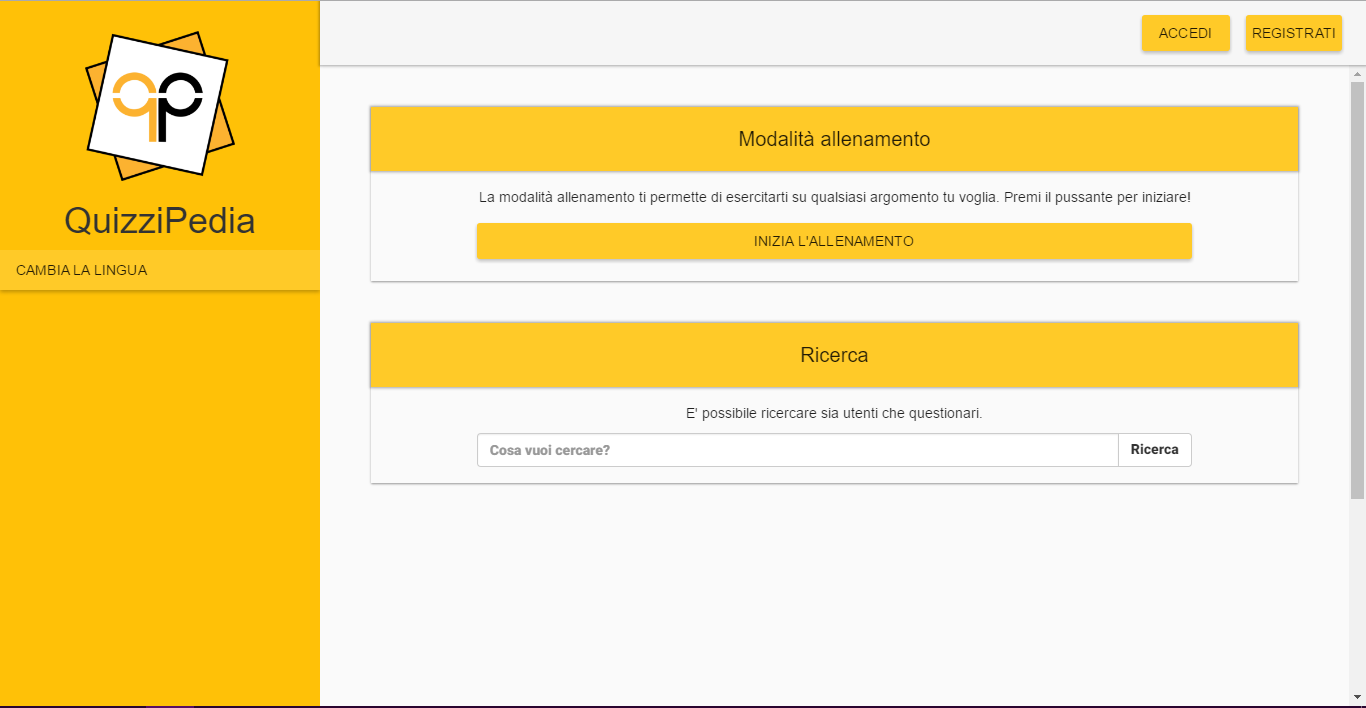
\includegraphics[scale=0.30]{img/homePage.png}
	\caption{Home Page}
\end{figure}
\FloatBarrier

L'Home Page di QuizziPedia presenta all'utente non ancora registrato le seguenti possibilità di utilizzo:
\begin{itemize}
	\item Registrazione;
	\item Autenticazione;
	\item Modalità allenamento;
	\item Ricerca utenti e questionari.
\end{itemize}
Le funzionalità \textit{Modalità allenamento} e \textit{Ricerca utenti e questionari} non necessitano di iscrizione al servizio, perciò l'utente non autenticato sarà libero di allenarsi in uno degli argomenti proposti e di ricercare i questionari e gli utenti presenti nel sistema.
\newpage
\section{Registrazione}

\label{Registrazione}
\begin{figure}[ht]
	\centering
	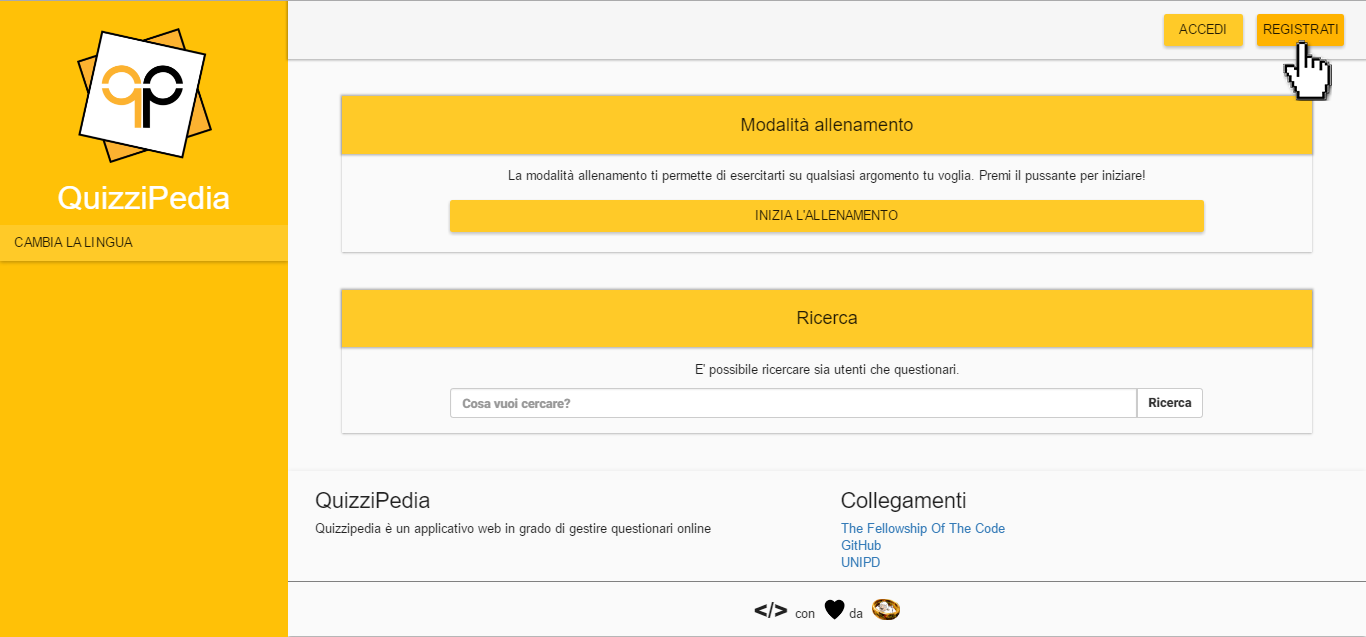
\includegraphics[scale=0.33]{img/vai_registrazione.png}
	\caption{Vai a Registrazione}
\end{figure}
\FloatBarrier

All'interno dell'Home Page è possibile accedere alla sezione \textit{Registrazione}. Una volta cliccato sul bottone apposito verrà presentata la seguente pagina:

\label{Registrazione_1}
\begin{figure}[ht]
	\centering
	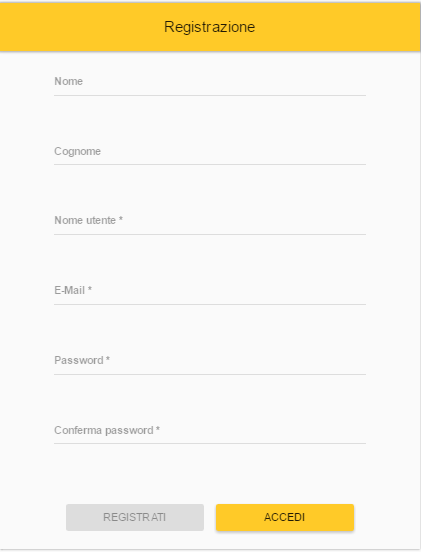
\includegraphics[scale=0.60]{img/registrazione.png}
	\caption{Registrazione}
\end{figure}
\FloatBarrier

L'utente per registrarsi deve obbligatoriamente compilare i seguenti campi:
\begin{itemize}
	\item Nome utente;
	\item E-mail;
	\item Password;
	\item Conferma password.
\end{itemize}
dove il campo \textit{Conferma password} deve essere identico al campo \textit{Password}, il quale deve avere almeno 8 caratteri. Compilati correttamente tutti i campi, il bottone \textit{Registrati}, prima disabilitato, permette di registrarsi effettuando un redirect alla pagina di autenticazione.  
\newpage
\section{Autenticazione}

\label{Autenticazione}
\begin{figure}[ht]
	\centering
	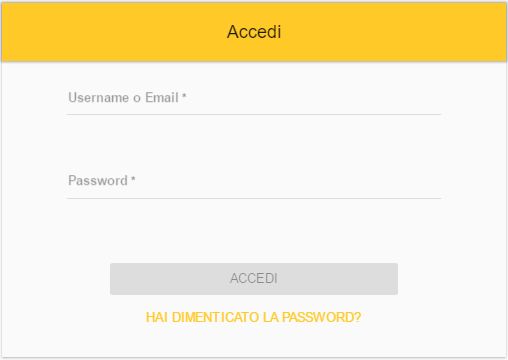
\includegraphics[scale=0.65]{img/autenticazione.png}
	\caption{Autenticazione}
\end{figure}
\FloatBarrier

Effettuata la registrazione è possibile autenticarsi al sistema. Compilati correttamente i campi \textit{Username o E-mail} e \textit{Password} il bottone \textit{Accedi} viene abilitato dando la possibilità di autenticarsi. Se l'autenticazione va a buon fine all'utente viene presentata l'Home Page con alcune nuove voci all'interno della barra del menù a destra. Se l'utente appena autenticato è di tipo normale saranno presenti le seguenti voci, le quali rappresentano le operazioni che l'utente è abilitato ad eseguire:
\begin{itemize}
	\item Gestione Profilo;
	\item Gestione domande;
	\item Cambia lingua.
\end{itemize}
Se invece l'utente è del tipo pro, gli verranno presentate le seguenti voci:
\begin{itemize}
	\item Gestione Profilo;
	\item Gestione questionari;
	\item Gestione domande;
	\item Cambia lingua. 
\end{itemize}
\newpage
\section{Modalità allenamento}
La \textit{Modalità allenamento} permette a qualsiasi tipo di utente di allenarsi in uno degli argomenti proposti dal sistema. Dopo aver cliccato sul pulsante \textit{INIZIA L'ALLENAMENTO} presente nell'Home Page, viene presentata la seguente pagina:

\label{Modalità allenamento}
\begin{figure}[ht]
	\centering
	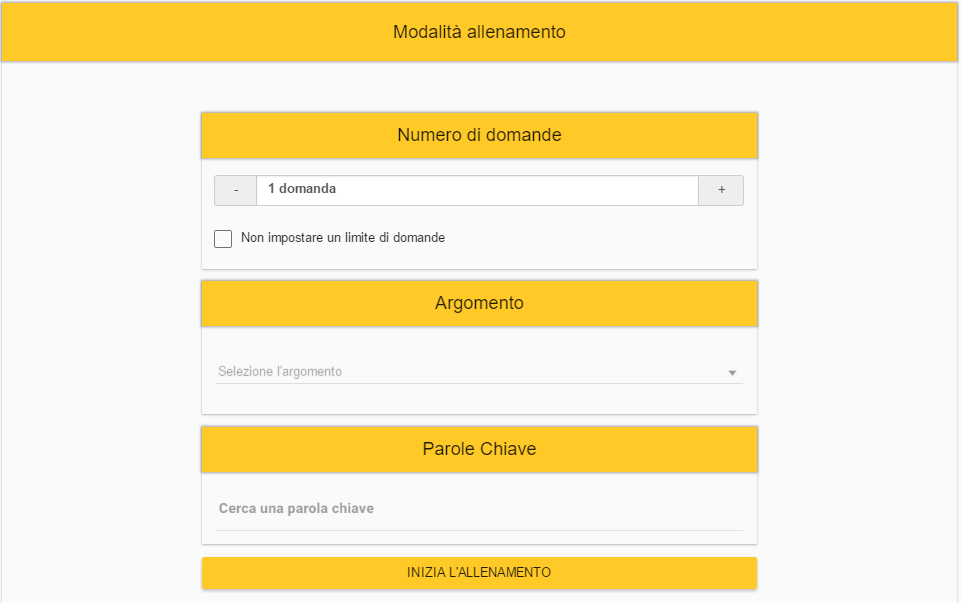
\includegraphics[scale=0.45]{img/allenamento.png}
	\caption{Modalità allenamento}
\end{figure}
\FloatBarrier

Prima di avviare un allenamento l'utente ha la possibilità di impostare i seguenti campi:
\begin{itemize}
	\item \textit{Numero di domande}: l'utente può impostare il numero massimo di domande che l'allenamento proporrà, oppure può decidere che non vi sia un limite prestabilito e avrà la possibilità di terminarlo quando vorrà;
	\item \textit{Argomento}: l'utente può selezionare l'argomento su cui verterà l'allenamento tra quelli proposti dal sistema;
	\item \textit{Parole chiave}: l'utente può ricercare le parole chiave a cui sono associate le domande e filtrarle così attraverso esse. Se ad esempio l'argomento selezionato è \textit{Patente} e la parola chiave ricercata è \textit{Guida}, il sistema proporrà domande relative all'argomento \textit{Patente} che hanno associata la parola chiave \textit{Guida}.
\end{itemize}

Terminata la compilazione dei campi sopra citati è possibile iniziare l'allenamento cliccando sul bottone \textit{INIZIA L'ALLENAMENTO}.
\newpage
\section{Visualizzazione profilo}
Dopo l'autenticazione, sarà possibile visualizzare i dati relativi al proprio profilo cliccando sulla prima voce del nuovo elenco presente sulla barra di sinistra:

\label{VaiProfilo}
\begin{figure}[ht]
	\centering
	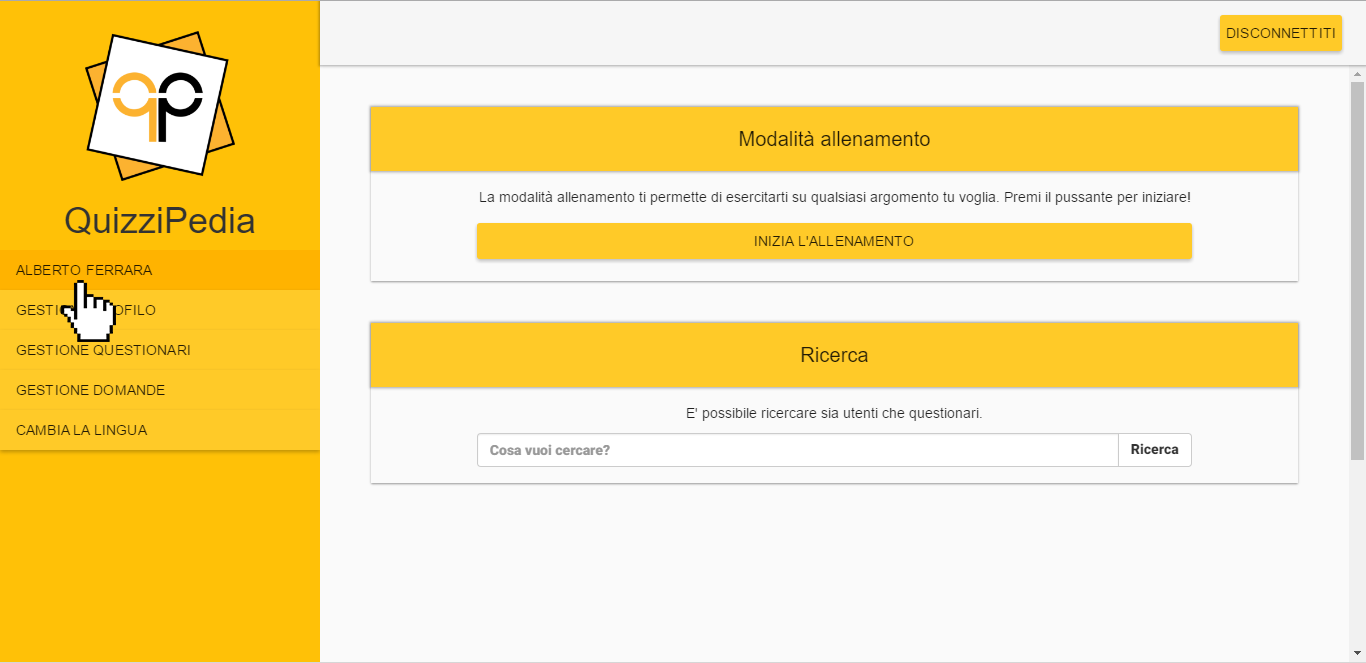
\includegraphics[scale=0.33]{img/vai_profilo.png}
	\caption{Vai a Visualizzazione profilo}
\end{figure}
\FloatBarrier

\newpage
Verrà presentata una pagina contenente tutti i dati relativi al proprio profilo utente. In particolare sarà possibile visualizzare la cronologia dei questionari svolti:

\label{CronologiaQuestionari}
\begin{figure}[ht]
	\centering
	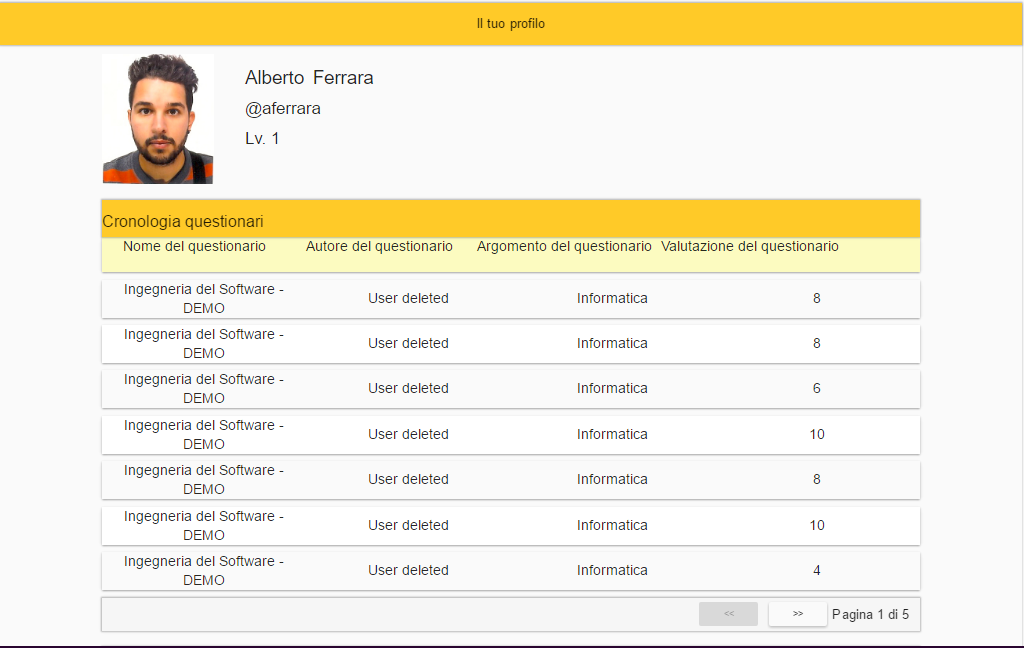
\includegraphics[scale=0.40]{img/cronologia_questionari.png}
	\caption{Cronologia questionari svolti}
\end{figure}
\FloatBarrier

i questionari approvati per la compilazione:
\begin{figure}[ht]
	\centering
	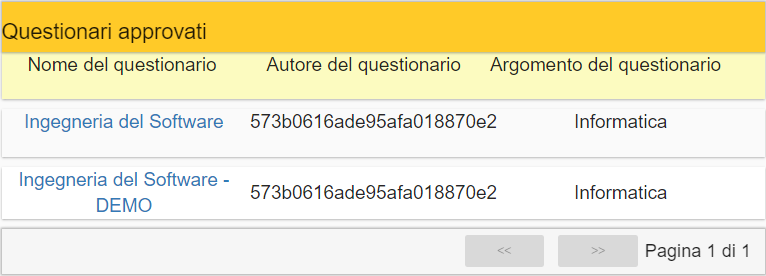
\includegraphics[scale=0.45]{img/questionari_approvati.png}
	\caption{Cronologia questionari svolti}
\end{figure}
\FloatBarrier

\newpage
i questionari a cui si è iscritti, ma non ancora abilitati alla compilazione: 

\label{QuestionariIscritto}
\begin{figure}[ht]
	\centering
	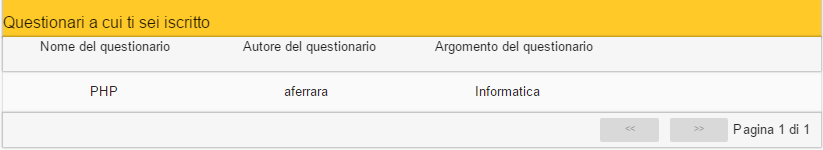
\includegraphics[scale=0.45]{img/questionari_iscritto.png}
	\caption{Questionari a cui si è iscritti}
\end{figure}
\FloatBarrier

e le proprie statistiche personali:

\label{StatistichePersonali}
\begin{figure}[ht]
	\centering
	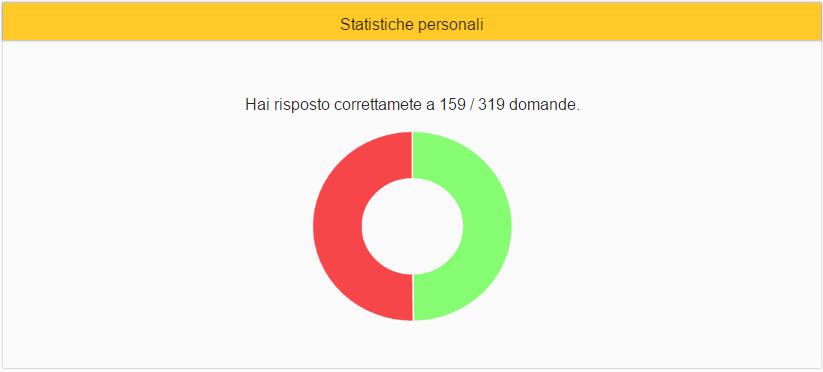
\includegraphics[scale=0.45]{img/statistiche_personali.png}
	\caption{Questionari a cui si è iscritti}
\end{figure}
\FloatBarrier
\newpage
\section{Gestione Profilo}
Il servizio permette ad un utente autenticato di aggiornare e/o modificare i propri dati personali. Cliccando la voce \textit{Gestione Profilo}, presente nella barra a sinistra, il sistema porta l'utente all'interno della pagina dedicata alla gestione del proprio profilo e account. All'interno di questa sezione è possibile:
\begin{itemize}
	\item Inserire un'immagine di profilo;
	\item Modificare il proprio nome;
	\item Modificare il proprio cognome;
	\item Modificare l'email;
	\item Inserire una nuova password.
\end{itemize}

\label{GestioneProfilo}
\begin{figure}[ht]
	\centering
	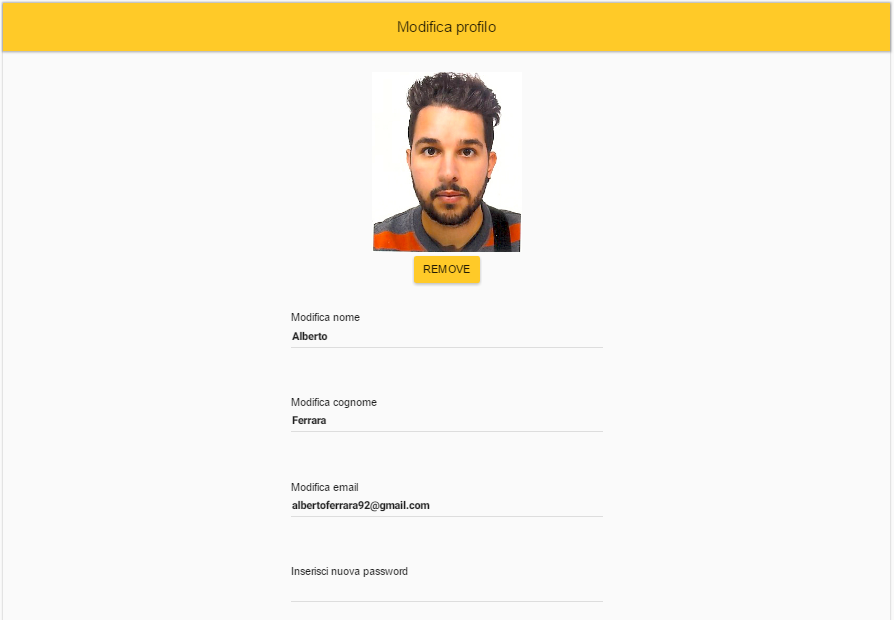
\includegraphics[scale=0.45]{img/gestione_profilo.png}
	\caption{Gestione profilo}
\end{figure}
\FloatBarrier


\paragraph{Gestione Questionari}

\label{Gestione Questionari - gestione del recupero dei questionari di un utente}

\begin{figure}[ht]
	\centering
	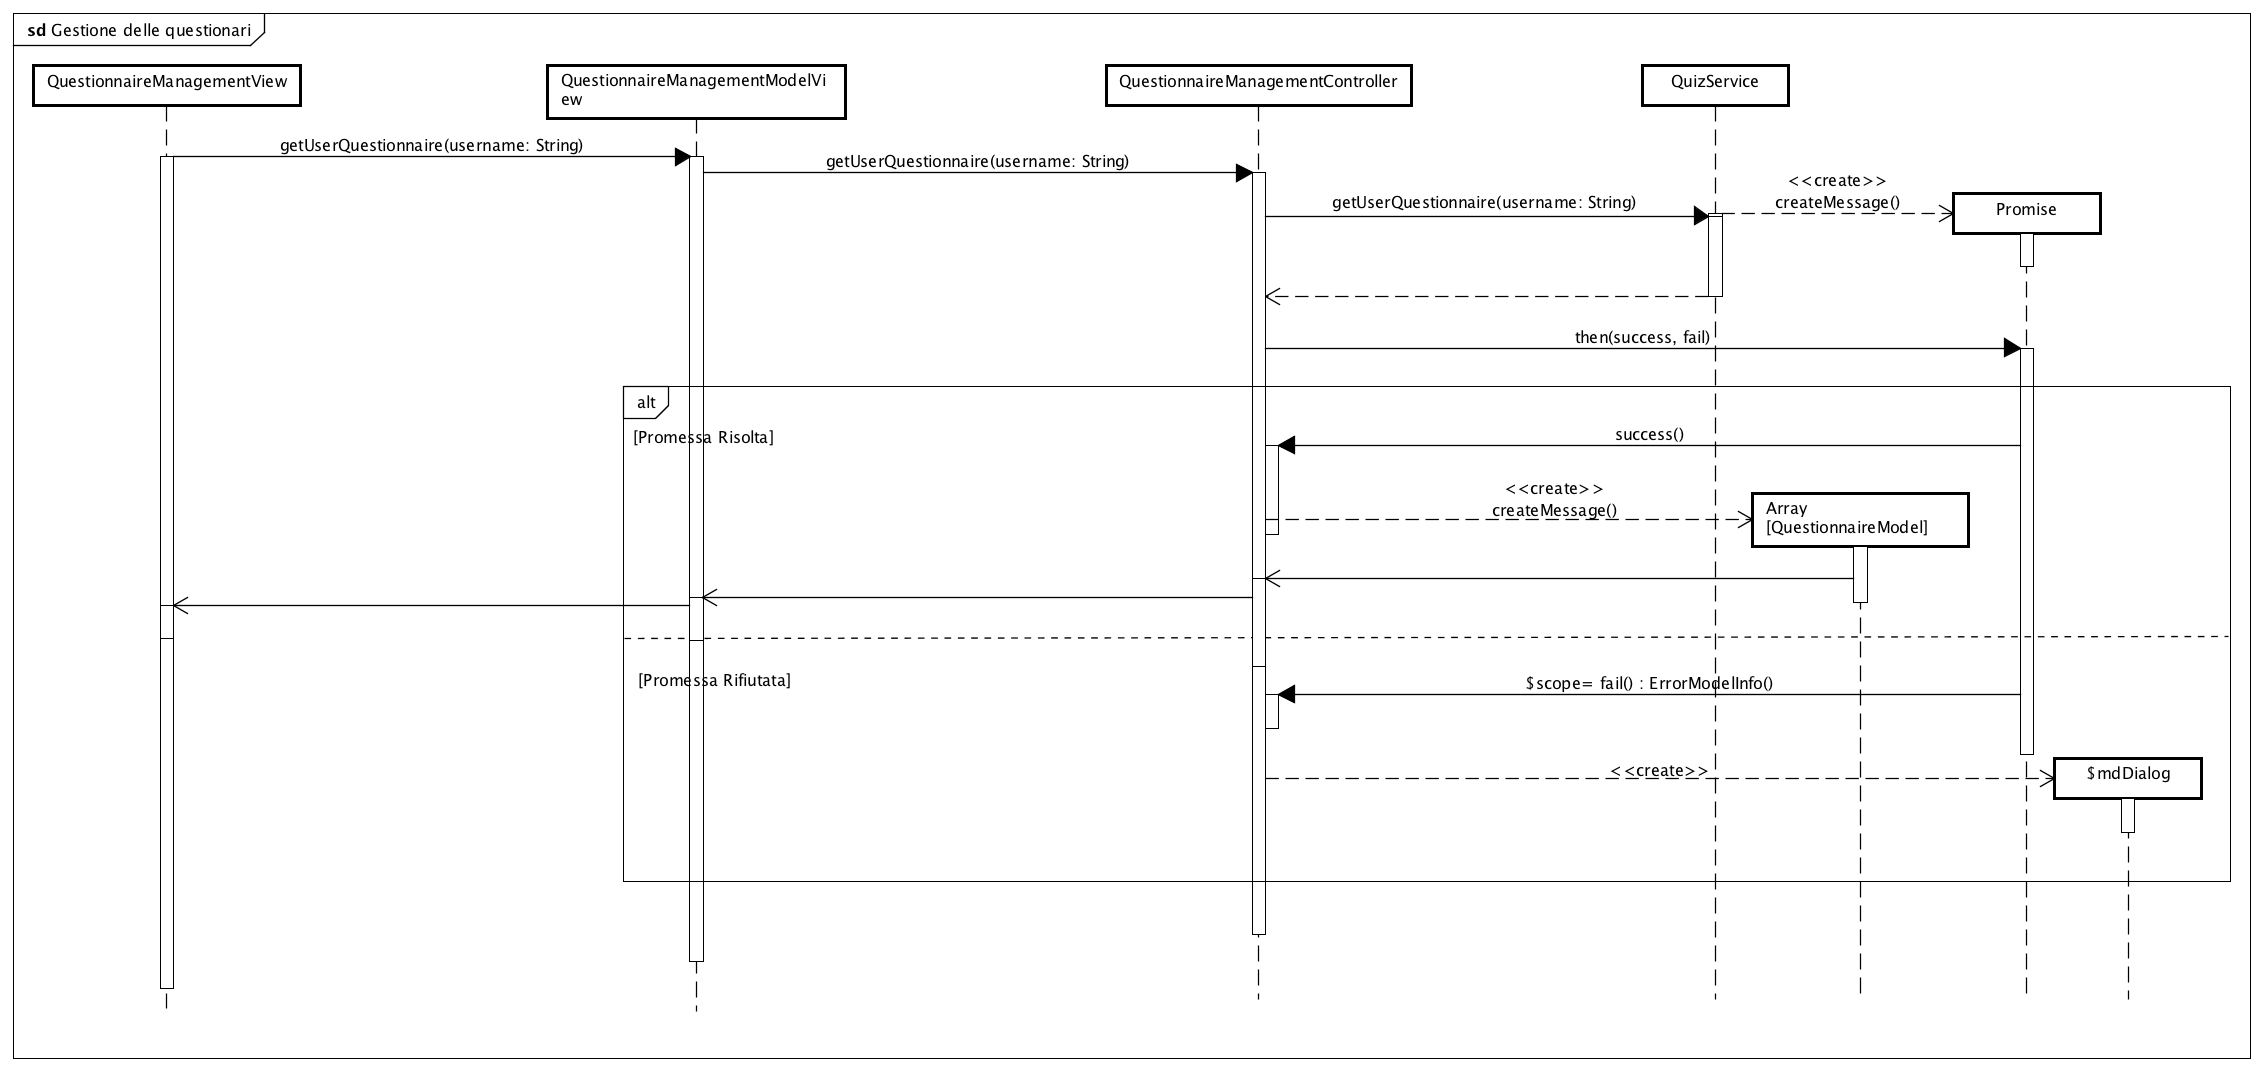
\includegraphics[scale=0.25,keepaspectratio]{UML/DiagrammiDiSequenza/Front-end/QuestionnaireManagement.png}
	\caption{Gestione Domande - gestione delle domande create da un utente}
\end{figure} \FloatBarrier

Nella view di visualizzazione domande verrà chiamato il metodo del controller che serve per ottenere tutti questionari create dall'utente autenticato. Il controller eseguirà una richiesta al service. A sua volta il service ritornerà una promise che potrà essere risolta o rifiutata. Nel caso venga risolta verrà ritornato l'array di tutti i questionari, nel caso invece venga rifiutata verrà restituito un oggetto contenente l'errore e visualizzato un messaggio informativo. 
\paragraph{Gestione Domande}

\label{Gestione delle domande create da un utente}

\begin{figure}[ht]
	\centering
	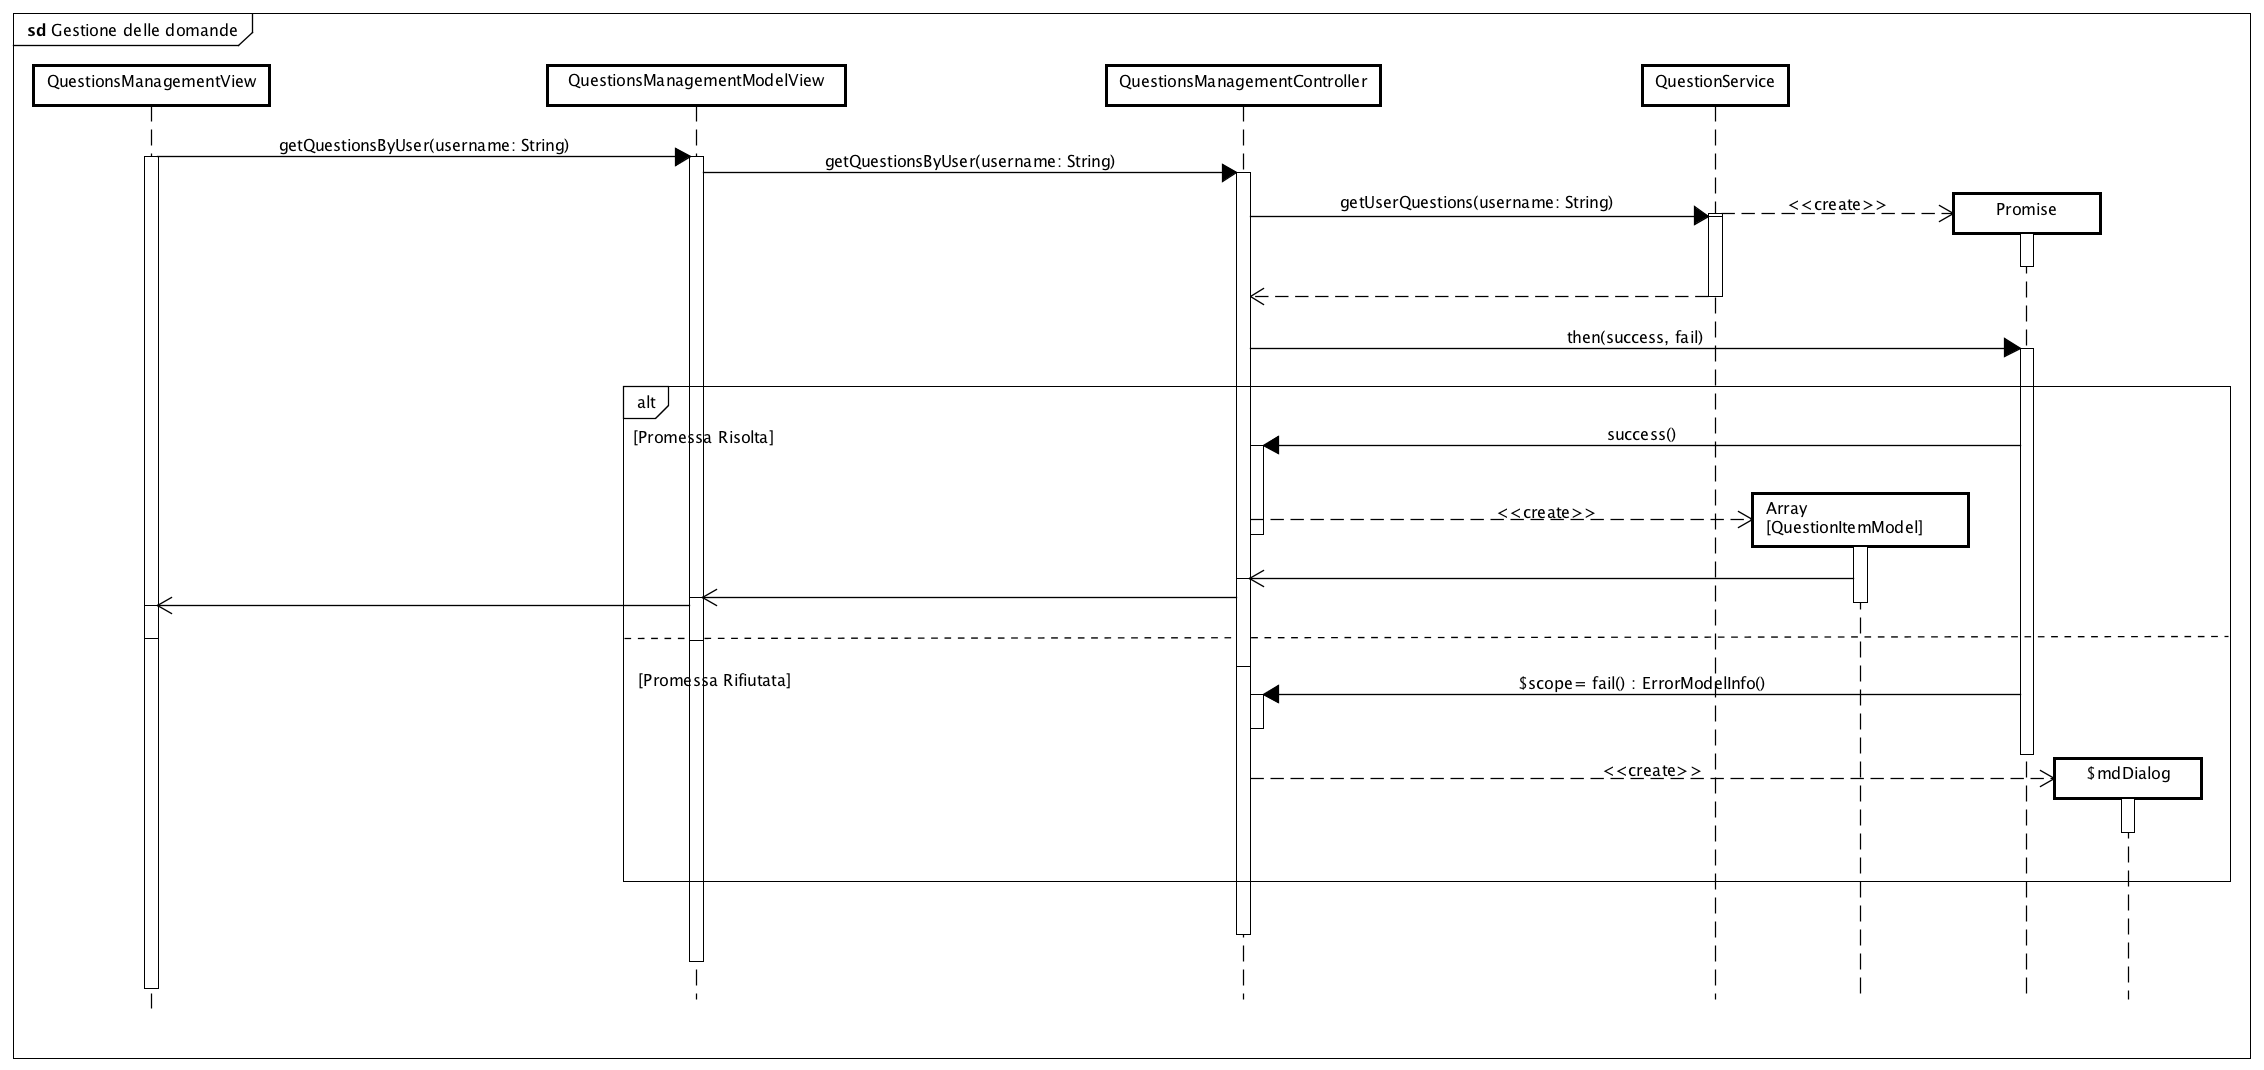
\includegraphics[scale=0.25,keepaspectratio]{UML/DiagrammiDiSequenza/Front-end/QuestionsManagement.png}
	\caption{Gestione delle domande create da un utente}
\end{figure} \FloatBarrier

Nella view di visualizzazione domande verrà chiamato il metodo del controller che serve per ottenere tutte le domande create dall'utente autenticato. Il controller eseguirà una richiesta al service. A sua volta il service ritornerà una promise che potrà essere risolta o rifiutata. Nel caso venga risolta verrà ritornato l'array di domande ottenuto dal back-end, nel caso invece venga rifiutata verrà restituito un oggetto contenente l'errore e visualizzato un messaggio informativo. 
\newpage
\section{Cambia lingua}
L'applicazione QuizziPedia è stata sviluppata in due differenti lingue: Italiano e Inglese. Per cambiare la lingua in uso basta selezionare la voce \textit{CAMBIA LINGUA} o \textit{CHANGE THE SYSTEM LANGUGE} dal menù a sinistra per far comparire così la seguente schermata:

 \label{CambiaLingua}
 \begin{figure}[ht]
 	\centering
 	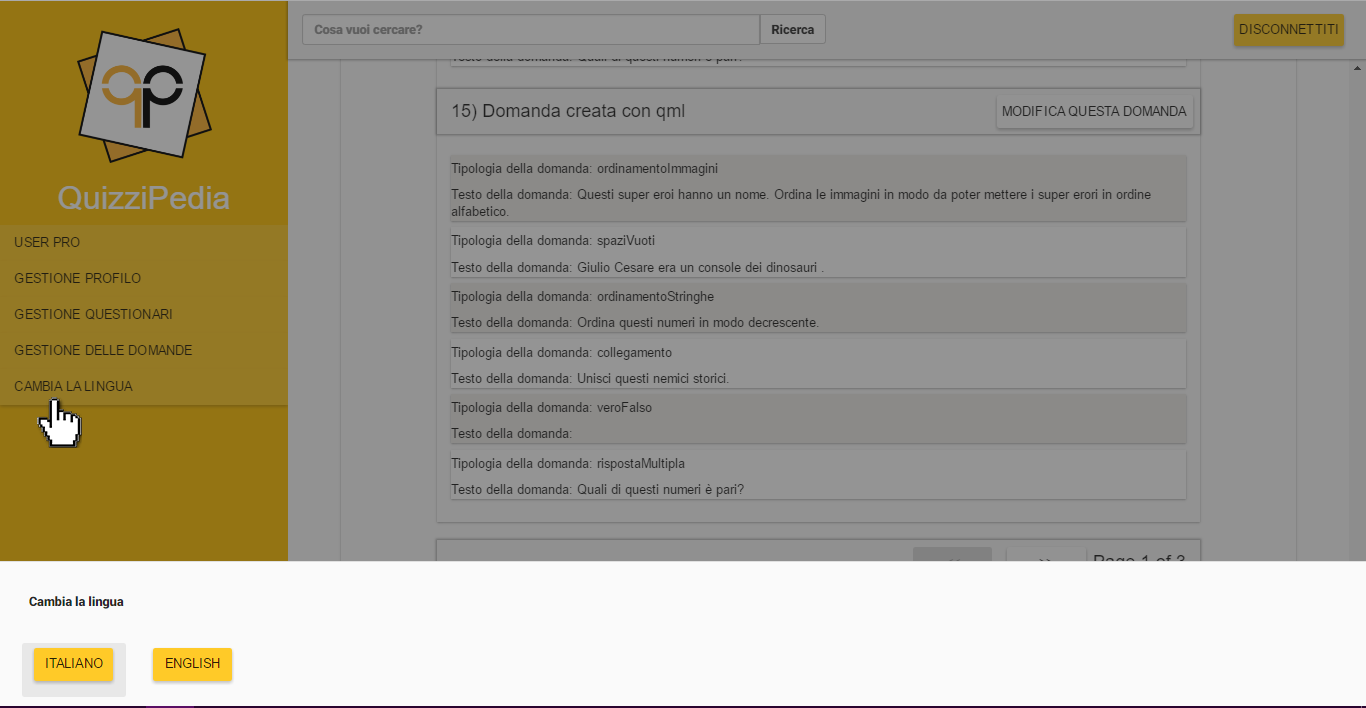
\includegraphics[scale=0.35]{img/cambia_lingua.png}
 	\caption{Cambia lingua}
 \end{figure}
 \FloatBarrier
\newpage
\section{Errori}
Durante l'utilizzo dell'applicazione QuizziPedia è possibile che l'utente incappi in alcuni errori presentati a video:

\label{Errore}
\begin{figure}[ht]
	\centering
	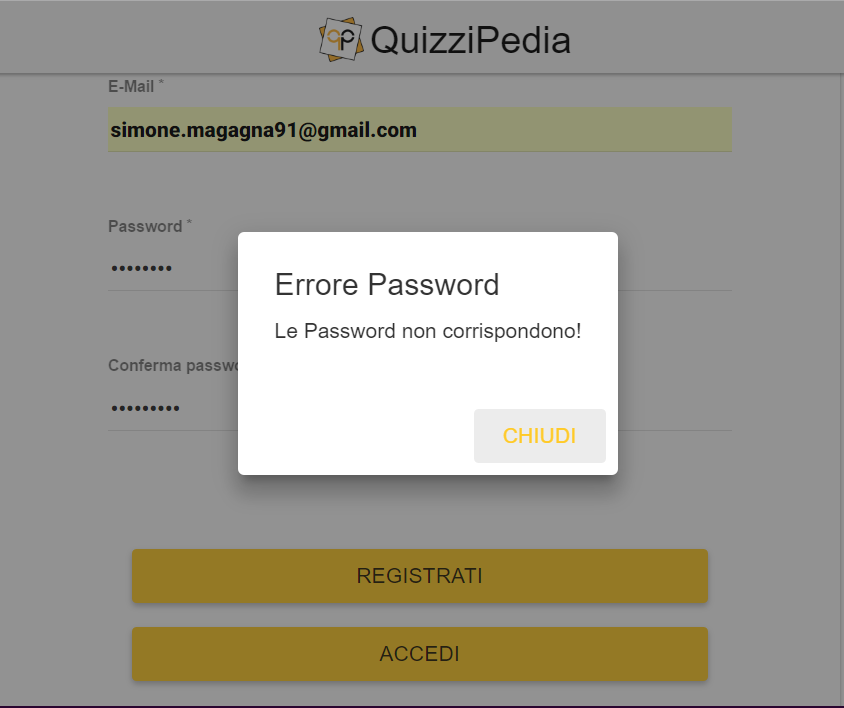
\includegraphics[scale=0.45]{img/errore.png}
	\caption{Errore: password non corrispondono}
\end{figure}
\FloatBarrier 

Viene ora presentata una lista contenente tutti i tipi di errore, con annessa descrizione, che un utente può trovare:

\begin{itemize}
	\item \texttt{Utente non trovato:} l'identificativo utente fornito non è un identificativo valido;
	\item \texttt{Credenziali non valide:} è necessario fornire un username ed una password valide;
	\item \texttt{Password assente:} è necessario inserire una password;
	\item \texttt{Password troppo corta:} è necessario inserire una password di almeno 8 caratteri;
	\item \texttt{Password uguale all'attuale:} è necessario inserire una password diversa della precedente;
	\item \texttt{Le password non coincidono:} è necessario che 'password' e 'conferma password' siano identiche;
	\item \texttt{Campo obbligatorio vuoto:} è necessario riempire tutti i campi obbligatori;
	\item \texttt{Username non disponibile:} l'username è già stato utilizzato, prego inserire un nuovo username;
	\item \texttt{Username non valido:} l'username non è valido;
	\item \texttt{Indirizzo mail non valido: } è necessario fornire un indirizzo e-mail valido;
	\item \texttt{Formato immagine non valido: } il formato dell'immagine non è valido;
	\item \texttt{Immagine di dimensione troppo grande: } la dimensione massima per l'immagine è di 20MB;
	\item \texttt{Caricamento immagine fallito}: errore sconosciuto nel caricamento dell'immagine;
	\item \texttt{Domanda non valida:} l'identificativo della domanda fornita non è un identificativo valido;
	\item \texttt{Argomento non valido:} l'identificativo dell'argomento fornito non è un identificativo valido;
	\item \texttt{Questionario non valido:}  l'identificativo del questionario fornito non è un identificativo valido;
	\item \texttt{Sommario non valido:} l'identificativo del sommario fornito non è un identificativo valido;
	\item \texttt{Contenuto domanda non valido:} i dati relativi al contenuto della domanda non sono  validi o sono formattati in modo errato;
	\item \texttt{Argomento non valido:} i dati relativi al contenuto dell'argomento non sono validi;
	\item \texttt{Contenuto questionario non valido:} i dati relativi al contenuto del questionario non sono validi;
	\item \texttt{Contenuto sommario non valido:} i dati relativi al contenuto del  sommario non sono validi o sono formattati in modo errato;
	\item \texttt{Dati modifica domanda non definiti:} i dati per la modifica di una domanda non sono definiti;
	\item \texttt{Argomento non definito:} i dati per la gestione dell'argomento non sono definiti;
	\item \texttt{Dati gestione questionario non definiti:} i dati per la gestione del questionario non sono definiti;
	\item \texttt{Sommario non valido:} i dati per la gestione del sommario non sono validi;
\end{itemize} 

\appendix
\newpage
\section{QML - Quiz Markup Language}
Uno dei punti fondamentali dell'applicazione è permettere agli utenti di poter creare domande da proporre negli allenamenti e nei questionari. Per rendere più semplice l'aggiunta di una domanda sono stati realizzati degli \textit{wizard\ped{G}} per alcune tipologie di domande, ma questo limita l'utente alla sola creazione di tali tipologie. La soluzione adottata è la realizzazione di un nuovo linguaggio di \textit{markup\ped{G}} che permette la definizione di domande non ordinarie, denominato QML acronimo di Quiz Markup Language.
Per la realizzazione di QML abbiamo adottato il \textit{Jison\ped{G}}, uno strumento che ci permette di definire un \textit{lexer\ped{G}} ed un \textit{parser\ped{G}} in grado di costruire e scorrere un albero di analisi al fine di generare un documento \texttt{JSON} a partire da una grammatica definita.

\subsection{Definizione della grammatica}
Per mantenere la semplicità di realizzazione di una domanda tramite QML è stato deciso di mantenere la sintassi \textit{JSON}, con l'aggiunta delle sole parole chiave necessarie per mantenere coerente la grammatica con lo scopo del QML. Alla grammatica è stata data possibilità di inserire commenti che saranno rimossi prima della creazione del \textit{JSON}.

\subsubsection{Sintassi domanda Vero/Falso}
\begin{lstlisting}[language=json,firstnumber=1]
{	
"type": "veroFalso",
"topic" : "Patente",
"image": "/img/veroFalso/example.png", //immagine possibile nel testo della domanda vero e falso
"answers":
	[{
	"text": "In Italia la guida e' a destra",
	"isItRight": true
	}],
"keywords":
	[{
	"guida",
	"legge",
	"italia"
	}] 
}
\end{lstlisting}

\subsubsection{Sintassi domanda a Risposta Multipla}
\begin{lstlisting}[language=json,firstnumber=1]
{	
"type" : "rispostaMultipla",
"topic" : "Matematica",
"questionText": "Quali di questi numeri e' pari?",
"url": "/img/rispostaMultipla/D0_3.png", //immagine possibile nel testo della domanda risposta multipla
"answers":
	[{
	"text": "1",
	"url": "/img/rispostaMultipla/D0_1.png", //url dell'immagine, possibile campo facoltativo
	"isItRight": false
	 },{
	"text": "2",
	"url": "/img/rispostaMultipla/D0_2.png", //url dell'immagine, possibile campo facoltativo
	"isItRight": true
	 },{
	"text": "7",
	"url": "/img/rispostaMultipla/D0_3.png", //url dell'immagine, possibile campo facoltativo
	"isItRight": false
	 },{
	"text": "9",
	"url": "/img/rispostaMultipla/D0_4.png", //url dell'immagine, possibile campo facoltativo
	"isItRight": false
	 }],
"keywords":
	[{
	"numeri",
	"matematica",
	"scuola"
	}]
}
\end{lstlisting}

\subsubsection{Sintassi domanda a Ordinamento di Stringhe}
\begin{lstlisting}[language=json,firstnumber=1]
{
"type": "ordinamentoStringhe",
"topic" : "Matematica",
"questionText": "Ordina questi numeri in modo decrescente.",
"answer":
	[{
	"text": "1",
	"position": 4
	},{
	"text": "2",
	"position": 3
	},{
	"text": "7",
	"position": 2
	},{
	"text": "9",
	"position": 1
	}],
"keywords":
	[{
	"ordinamento",
	"numeri",
	}]
}
\end{lstlisting}

\subsubsection{Sintassi domanda a Ordinamento Immagini}
\begin{lstlisting}[language=json,firstnumber=1]
{
"type": "ordinamentoImmagini",
"topic" : "Grammatica Italiana",
"questionText": "Ordina queste immagini in modo da ottenere la parola "CIAO".",
"url": "/img/ordinamentoImmagini/D0_1.png", //immagine possibile nel testo della domanda ad ordianamento di immagini
"answer":
	[{
	"url": "/img/domandeOrdinamentoImmagini/I.png", //url dell'immagine
	"position": 2
	},{
	"url": "/img/domandeOrdinamentoImmagini/A.png",
	"position": 3
	},{
	"url": "/img/domandeOrdinamentoImmagini/O.png",
	"position": 4
	},{
	"url": "/img/domandeOrdinamentoImmagini/C.png",
	"position": 1
	}],
"keywords":
	[{
	"parole",
	"grammatica"
	}]
}
\end{lstlisting}

\subsubsection{Sintassi domanda a Collegamento di Elementi}
\begin{lstlisting}[language=json,firstnumber=1]
{
"type": "collegamentoElementi",
"topic" : "Cultura Generale",
"questionText": "Collega queste coppie di nemici classici.",
"answer":
	[{
	"text_1_A": "cane",
	"text_1_B": "gatto"
	},{
	"url_2_A": "/img/collegamento/uncino.png",
	"text_2_B": "peter pan"
	},{
	"url_3_A": "/img/collegamento/D0_1.png",
	"url_3_B": "/img/collegamento/D0_5.png"
	}],
"keywords":
	[{
	"nemici"
	}]
}
\end{lstlisting}

\subsubsection{Sintassi domanda ad Area Cliccabile}
\begin{lstlisting}[language=json,firstnumber=1]
{
"type": "areaCliccabile",
"topic" : "Medicina",
"questionText": "Clicca quale tra le seguenti scelte e' il bicipide.",
"image": "/img/areaCliccabile/D0_1.png", //sfondo dell'area cliccabile
"resolution": { "x":400, "y":500 },
"answer":
	[{
	"x": "200",
	"y": "50",
	"text": "testo facoltativo di arricchimento"
	},{
	"x": "300",
	"y": "120",
	"text": "testo facoltativo di arricchimento"
	},{
	"x": "200",
	"y": "200",
	"text": "testo facoltativo di arricchimento"
	}],
"keywords":
	[{
	"corpo umano",
	"medicina",
	"scienze" ,
	"muscoli"
	}]
}
\end{lstlisting}

\subsubsection{Sintassi domanda a Riempimento spazi vuoti}
\begin{lstlisting}[language=json,firstnumber=1]
{
"type": "spaziVuoti",
"topic" : "Storia"
"questionText": "Giulio Cesare era un console romano.",
"answer":
	[{
	"parolaNumero": 2 //sta ad indicare quale parola e' da oscurare. In questo caso la numero 2
	},{
	"parolaNumero": 5
	}],
"keywords":
	[{
	"storia",
	}] 
}
\end{lstlisting}

\subsection{Generazione del JSON}
Se il \textit{parser\ped{G}} non trova errori o ambiguità viene creato un \textit{JSON\ped{G}} contente la domanda e altre informazioni necessarie per aggiungerla al sistema. Ogni tipologia di domanda crea un tipo di \textit{JSON\ped{G}} diverso, questo accada sia per la generazione tramite \textit{wizard\ped{G}} sia tramite QML.

\subsubsection{JSON domanda Vero/Falso}
\begin{lstlisting}[language=json,firstnumber=1]
{
"author" : "__userId",
"makeWith" : "QML" || "wizzard" ,
"language" : "it || en",
"question" :
	[{
	"type": "veroFalso",
	"image": "/img/veroFalso/example.png", //immagine possibile nel testo della domanda vero e falso
	"answers":
		[{
		"text": "In Italia la guida e' a destra",
		"isItRight": true
		}]
	}],
"keywords" : 
	[{
	"guida",
	"legge",
	"italia"
	}],
"level" : 500,
"totalAnswers" : 0,
"correctAnswers" : 0
}
\end{lstlisting}

\subsubsection{JSON domanda a Risposta Multipla}
\begin{lstlisting}[language=json,firstnumber=1]
{	
"author" : "_UserId",
"makeWith" : "QML" || "wizzard" ,
"language" : "it || en" ,
"type": "rispostaMultipla",
"question" [{
	"questionText": "Quali di questi numeri e' pari?",
	"url": "/img/rispostaMultipla/D0_3.png", //immagine possibile nel testo della domanda risposta multipla
	"answers":
		[{
		"text": "1",
		"url": "/img/rispostaMultipla/D0_1.png", //url dell'immagine, possibile campo facoltativo
		"isItRight": false
		},{
		"text": "2",
		"url": "/img/rispostaMultipla/D0_2.png", //url dell'immagine, possibile campo facoltativo
		"isItRight": true
		},{
		"text": "7",
		"url": "/img/rispostaMultipla/D0_3.png", //url dell'immagine, possibile campo facoltativo
		"isItRight": false
		},{
		"text": "9",
		"url": "/img/rispostaMultipla/D0_4.png", //url dell'immagine, possibile campo facoltativo
		"isItRight": false
		}]
}],
"keywords":
	[{
	"numeri",
	"matematica",
	"scuola"
	}],
"level" : 500,
"totalAnswers" : 0,
"correctAnswers" : 0
}
\end{lstlisting}

\subsubsection{JSON domanda a Ordinamento di Stringhe}
\begin{lstlisting}[language=json,firstnumber=1]
{
"author" : "_UserId", 
"makeWith" : "QML" || "wizzard" ,
"language" : "it || en",
"question" : [{
	"type": "ordinamentoStringhe",
	"questionText": "Ordina questi numeri in modo decrescente.",
	"answers":
		[{
		"text": "1",
		"position": 4
		},{
		"text": "2",
		"position": 3
		},{
		"text": "7",
		"position": 2
		},{
		"text": "9",
		"position": 1
		}]
}],
"keywords":
	[{
	"ordinamento",
	"numeri",
	}],
"level" : 500,
"totalAnswers" : 0,
"correctAnswers" : 0
}
\end{lstlisting}

\subsubsection{JSON domanda a Ordinamento Immagini}
\begin{lstlisting}[language=json,firstnumber=1]
{
"author" : "_UserId",
"makeWith" : "QML" || "wizzard" ,
"language" : "it || en",
"question" : [{
	"type": "ordinamentoImmagini",
	"questionText": "Ordina queste immagini in modo da ottenere la parola "CIAO".",
	"url": "/img/ordinamentoImmagini/D0_1.png", //immagine possibile nel testo della domanda ad ordianamento di immagini
	"answers":
		[{
		"url": "/img/domandeOrdinamentoImmagini/I.png", //url dell'immagine
		"position": 2
		},{
		"url": "/img/domandeOrdinamentoImmagini/A.png",
		"position": 3
		},{
		"url": "/img/domandeOrdinamentoImmagini/O.png",
		"position": 4
		},{
		"url": "/img/domandeOrdinamentoImmagini/C.png",
		"position": 1
		}]
}],
"keywords":
	[{
	"parole",
	"grammatica"
	}],
"level" : 500,
"totalAnswers" : 0,
"correctAnswers" : 0
}
\end{lstlisting}

\subsubsection{JSON domanda a Collegamento di Elementi}
\begin{lstlisting}[language=json,firstnumber=1]
{
"author" : "_UserId",
"makeWith" : "QML" || "wizzard" ,
"language" : "it || en",
"question" : [{
	"type": "collegamento",
	"questionText": "Collega queste coppie di nemici classici.",
	"answers":
		[{
		"text_1_A": "cane",
		"text_1_B": "gatto"
		},{
		"url_2_A": "/img/collegamento/uncino.png",
		"text_2_B": "peter pan"
		},{
		"url_3_A": "/img/collegamento/D0_1.png",
		"url_3_B": "/img/collegamento/D0_5.png"
		}]
}],
"keywords":
	[{
	"nemici"
	}],
"level" : 500,
"totalAnswers" : 0,
"correctAnswers" : 0
}
\end{lstlisting}

\subsubsection{JSON domanda ad Area Cliccabile}
\begin{lstlisting}[language=json,firstnumber=1]
{
"author" : "_UserId" ,
"makeWith" : "QML" || "wizzard" ,
"language" : "it || en", 
"question" : [{
	"type": "areaCliccabile",
	"questionText": "Clicca quale tra le seguenti scelte e' il bicipide.",
	"image": "/img/areaCliccabile/D0_1.png", //sfondo dell'area cliccabile
	"resolution": { "x":400, "y":500 },
	"answers":
		[{
		"x": "200",
		"y": "50",
		"text": "testo facoltativo di arricchimento"
		},{
		"x": "300",
		"y": "120",
		"text": "testo facoltativo di arricchimento"
		},{
		"x": "200",
		"y": "200",
		"text": "testo facoltativo di arricchimento"
		}]
}],
"keywords":
	[{
	"corpo umano",
	"medicina",
	"scienze" ,
	"muscoli"
	}],
"level" : 500,
"totalAnswers" : 0,
"correctAnswers" : 0
}
\end{lstlisting}

\subsubsection{JSON domanda a Riempimento spazi vuoti}
\begin{lstlisting}[language=json,firstnumber=1]
{
"author" : "_UserId",
"makeWith" : "QML" || "wizzard",
"language" : "it || en",
"question" : [{
	"type": "spaziVuoti",
	"questionText": "Giulio Cesare era un console romano.",
	"answers":
		[{
		"parolaNumero": 2 //sta ad indicare quale parola e' da oscurare. In questo caso la numero 2
		},{
		"parolaNumero": 5
		}]
}],
"keywords":
	[{
	"storia",
	}],
"level" : 500,
"totalAnswers" : 0,
"correctAnswers" : 0
}
\end{lstlisting}

%Generazione delle variabili che andranno a sostituire quelle del template `HomePage.tex`
\newcommand{\documento}{\G}
\newcommand{\nomedocumentofisico}{Glossario.pdf}
\newcommand{\redazione}{\SM}
\newcommand{\verifica}{\FB}
\newcommand{\approvazione}{Da Approvare}
\newcommand{\uso}{Esterno}
\newcommand{\destinateTo}{\TV \\ & \RC \\ & \proponente \\ & \gruppo}
\newcommand{\datacreazione}{24 Dicembre 2015}
\newcommand{\datamodifica}{24 Dicembre 2015}
\newcommand{\stato}{Sviluppo}

\def\TABELLE{false}	%abilita - disabilita l'indice delle tabelle
\def\FIGURE{false} 	%abilita - disabilita l'indice delle figure

\documentclass[a4paper,11pt]{article}

%***IMPORTAZIONE PACKAGE***
\usepackage{ifthen}
\usepackage[italian]{babel}
\usepackage[utf8]{inputenc}
\usepackage[T1]{fontenc}
\usepackage{float}
\usepackage{chapterbib}
\usepackage{graphicx}
\usepackage[a4paper,top=2.5cm,bottom=2.5cm,left=2.5cm,right=2.5cm]{geometry}
\usepackage[colorlinks=true, urlcolor=black, citecolor=black, linkcolor=black]{hyperref}
\usepackage{booktabs}
\usepackage{fancyhdr}
\usepackage{totpages}
\usepackage{tabularx, array}
\usepackage{dcolumn}
\usepackage{epstopdf}
\usepackage{booktabs}
\usepackage{fancyhdr}
\usepackage{longtable}
\usepackage{calc}
\usepackage{datatool}
\usepackage[bottom]{footmisc}
\usepackage{listings} 
\usepackage{textcomp}
\usepackage{titlesec}
\usepackage{rotating} 
\usepackage{multirow}
\usepackage{placeins}
\usepackage{color}
\usepackage[table,usenames,dvipsnames]{xcolor}
\usepackage{hyperref}
\usepackage{makecell}
\usepackage{hyperref}


%***STILE PAGINA***
\pagestyle{fancy}
%no indentazione paragrafo
\setlength{\parindent}{0pt}

%***INTESTAZIONE***
\lhead{\Large{\progetto} \\ \footnotesize{\documento}}
\rhead{
\includegraphics[keepaspectratio = true, width = 25px] {../../Template/icone/LogoGruppo.png}}
\renewcommand{\headrulewidth}{0.4pt}  %Linea sotto l'intestazione

%***PIÈ DI PAGINA***
\lfoot{\textit{\gruppoLink}\\ \footnotesize{\email}}
\rfoot{\thepage} %per le prime pagine: mostra solo il numero romano
\cfoot{}
\renewcommand{\footrulewidth}{0.4pt}   %Linea sopra il piè di pagina

%***INSERIMENTO DI NUOVE SOTTOSEZIONI
\setcounter{secnumdepth}{7}		% mostra nel documento fino al livello 8 (1.2.3.4.5.6.7.8)
\setcounter{tocdepth}{7}			% mostra nell'indice fino al livello 8 (1.2.3.4.5.6.7.8)

%***LA SOTTOSEZIONE PARAGRAPH VIENE VISUALIZZATA COME UNA SECTION
\titleformat{\paragraph}{\normalfont\normalsize\bfseries}{\theparagraph}{1em}{}
\titlespacing*{\paragraph}{0pt}{3.25ex plus 1ex minus .2ex}{1.5ex plus .2ex}

\titleformat{\subparagraph}{\normalfont\normalsize\bfseries}{\thesubparagraph}{1em}{}
\titlespacing*{\subparagraph}{0pt}{3.25ex plus 1ex minus .2ex}{1.5ex plus .2ex}

\makeatletter
\newcounter{subsubparagraph}[subparagraph]
\renewcommand\thesubsubparagraph{%
  \thesubparagraph.\@arabic\c@subsubparagraph}
\newcommand\subsubparagraph{%
  \@startsection{subsubparagraph}    % counter
    {6}                              % level
    {\parindent}                     % indent
    {3.25ex \@plus 1ex \@minus .2ex} % beforeskip
    {0.75em}                           % afterskip
    {\normalfont\normalsize\bfseries}}
\newcommand\l@subsubparagraph{\@dottedtocline{6}{10em}{5.5em}} %gestione dell'indice
\newcommand{\subsubparagraphmark}[1]{}
\makeatother

\makeatletter
\newcounter{subsubsubparagraph}[subsubparagraph]
\renewcommand\thesubsubsubparagraph{%
  \thesubsubparagraph.\@arabic\c@subsubsubparagraph}
\newcommand\subsubsubparagraph{%
  \@startsection{subsubsubparagraph}    % counter
    {7}                              % level
    {\parindent}                     % indent
    {3.25ex \@plus 1ex \@minus .2ex} % beforeskip
    {0.75em}                           % afterskip
    {\normalfont\normalsize\bfseries}}
\newcommand\l@subsubsubparagraph{\@dottedtocline{7}{10em}{6.5em}} %gestione dell'indice
\newcommand{\subsubsubparagraphmark}[1]{}
\makeatother
%Generali
\newcommand{\progetto}{QuizziPedia}
\newcommand{\gruppo}{TheFellowshipOfTheCode}
\newcommand{\gruppoLink}{\href{http://thefellowshipofthecode.github.io/}{TheFellowshipOfTheCode}}
\newcommand{\email}{\href{mailto:thefellowshipofthecode@gmail.com}{thefellowshipofthecode@gmail.com}}

%Documenti
\newcommand{\AdR}{Analisi dei Requisiti}
\newcommand{\NdP}{Norme di Progetto}
\newcommand{\PdP}{Piano di Progetto}
\newcommand{\SdF}{Studio di Fattibilità}
\newcommand{\PdQ}{Piano di Qualifica}
\newcommand{\VI}{Verbale Interno}
\newcommand{\VE}{Verbale Esterno}
\newcommand{\ST}{Specifica Tecnica}
\newcommand{\DDP}{Definizione di Prodotto}
\newcommand{\MU}{Manuale Utente}
\newcommand{\G}{Glossario}
\newcommand{\LdP}{Lettera di Presentazione}
\newcommand{\NdPv}{NormeDiProgetto\_v\_1\_0\_0}
\newcommand{\PdPv}{PianoDiProgetto\_v\_1\_0\_0}
\newcommand{\PdQv}{PianoDiQualifica\_v\_1\_0\_0}
\newcommand{\SdFv}{StudioDiFattibilità\_v\_1\_0\_0}

%Componenti del gruppo
\newcommand{\AF}{Alberto Ferrara}
\newcommand{\SM}{Simone Magagna}
\newcommand{\FB}{Franco Berton}
\newcommand{\MP}{Marco Prelaz}
\newcommand{\MV}{Mattia Varotto}
\newcommand{\GN}{Matteo Gnoato}
\newcommand{\GR}{Matteo Granzotto}

%Ruoli
\newcommand{\RdP}{Responsabile di Progetto}
\newcommand{\Res}{Responsabile}
\newcommand{\Amm}{Amministratore}
\newcommand{\Ver}{Verificatore}
\newcommand{\Prog}{Progettista}
\newcommand{\Progr}{Programmatore}
\newcommand{\Ana}{Analista}
\newcommand{\RdPs}{Responsabili di Progetto}
\newcommand{\Ress}{Responsabile}
\newcommand{\Amms}{Amministratori}
\newcommand{\Vers}{Verificatori}
\newcommand{\Progs}{Progettisti}
\newcommand{\Progrs}{Programmatori}
\newcommand{\Anas}{Analisti}

%Professori e proponente
\newcommand{\TV}{Prof. Tullio Vardanega}
\newcommand{\RC}{Prof. Riccardo Cardin}
\newcommand{\ZU}{Zucchetti S.P.A.}
\newcommand{\proponente}{Zucchetti S.P.A.}

\newcommand{\diaryEntry}[5]{#2 & \emph{#4} & #3 & #5 & #1\\ \hline}

%comando per una nuova riga nella tabella del diario delle modifiche
\newcommand{\specialcell}[2][c]{%
	\begin{tabular}[#1]{@{}c@{}}#2\end{tabular}}

\renewcommand*\sectionmark[1]{\markboth{#1}{}}
\renewcommand*\subsectionmark[1]{\markright{#1}}

%Pediodi di lavoro 
\newcommand{\AR}{Analisi dei Requisiti}
\newcommand{\AD}{Analisi dei Requisiti in Dettaglio}
\newcommand{\PA}{Progettazione Architetturale}
\newcommand{\PD}{Progettazione di Dettaglio}
\newcommand{\CO}{Codifica}
\newcommand{\VV}{Verifica e Validazione}

% Revisioni
\newcommand{\RR}{Revisione dei Requisiti}
\newcommand{\RP}{Revisione di Progettazione}
\newcommand{\RQ}{Revisione di Qualifica}
\newcommand{\RA}{Revisione di Accettazione}

% Comandi analisi dei requisiti
\newcommand{\uau}{utente autenticato}
\newcommand{\uaus}{utenti autenticati}
\newcommand{\uaupro}{utente autenticato pro}
\newcommand{\uauspro}{utenti autenticati pro}

\newcommand{\myincludegraphics}[2][]{%
	\setbox0=\hbox{\phantom{X}}%
	\vtop{
		\hbox{\phantom{X}}
		\vskip-\ht0
		\hbox{\includegraphics[#1]{#2}}}}


\newcommand{\modificheuno} 
{	
	0.0.3 & Inseriti i primi riferimenti informativi & \specialcell[t]{\GN \\ \prog} & 2016-02-26
	\\\midrule
	0.0.2 & Stesura scopo del documento, scopo del prodotto , riferimenti normativi & \specialcell[t]{\GN \\ \prog} & 2016-02-26
	\\\midrule
	0.0.1 & Creato template documento & \specialcell[t]{\GN \\ \prog} & 2016-02-26
	\\\midrule
}
\newcommand{\modifichedue}
{
}
%Serve per vedere i paragraph nell'indice
\setcounter{secnumdepth}{7}
\setcounter{tocdepth}{7}
\begin{document}

%inclusione template HomePage
\begin{center}

%
\includegraphics[width=1em]{../../../Template/icone/LogoGruppo.png}
\begin{large} \textbf{\gruppoLink} \end{large}
%
\includegraphics[width=1em]{../../../Template/icone/LogoGruppo.png}
\vspace{0.2em}

\hrule
\vspace{3em}


\includegraphics[keepaspectratio = true, width=8cm]{../../../Template/icone/LogoGruppo.png}

%Prima pagina senza intestazione né piè di pagina	
\thispagestyle{empty}

%Le informazioni del documento sono ancorate a fine pagina
\vfill

%Copertina
\begin{center} 
  \begin{Huge}
  {\fontsize{15mm}{20mm}\selectfont \progetto} 
  \end{Huge}
\end{center}

\begin{Huge} \documento \end{Huge}

\begin{center}
\textbf{Informazioni sul documento} \\ \vspace{2em}
\small
\begin{tabular}{r|l}
	\textbf{Nome Documento} & \nomedocumentofisico \\
	\textbf{Versione}	& 1\\
	\textbf{Data di Creazione} & \datacreazione\\
	\textbf{Data ultima modifica} & \datamodifica\\
	\textbf{Stato} & \stato \\
	\textbf{Redazione}	& \redazione\\
	\textbf{Verifica}	& \verifica\\
	\textbf{Approvazione}	& \approvazione\\
	\textbf{Uso}  & \uso\\
	\textbf{Distribuzione} & \gruppo \\
	\textbf{Destinato a}  &  \destinateTo \\
	\textbf{Email di riferimento} & \email
\end{tabular}
\end{center}

\normalsize
%Sommario
\textbf{Sommario\\} 
Documento contenente le norme di progetto che il gruppo \textit{\gruppo} seguirà durante tutte le fasi di realizzazione del prodotto \textit{\progetto}.

%\vfill %cosa fa?
\end{center}
\clearpage


%Registro delle modifiche e indice 
%si usa la numerazione romana per gli indici e la tabella delle modifiche
\pagenumbering{Roman}
\newpage
%***REGISTRO DELLE MODIFICHE***
%Vari comandi per la struttura della tabella, NON MODIFICARE!
\begin{center}
	\Large{\textbf{Registro delle modifiche}}
	\\\vspace{0.5cm}
	\normalsize
	\begin{tabularx}{\textwidth}{cXcc}
		\textbf{Versione} & \textbf{Descrizione} & \textbf{Autore e Ruolo} & \textbf{Data} \\\toprule
		\modifiche
		\bottomrule
\end{tabularx}
\end{center}
\newpage
%Inserisce il link all'indice
%\addcontentsline{toc}{section}{Indice}
\tableofcontents
\clearpage 

%Se è stata impostata a true la variabile per la lista delle tabelle, la mostra
\ifthenelse{\equal{\TABELLE}{true}} 
{\listoftables \newpage}{}

%Se è stata impostata a true la variabile per la lista delle figure, la mostra
\ifthenelse{\equal{\FIGURE}{true}}
{\listoffigures \newpage}{}

%Da qui comincia la numerazione normale
\pagenumbering{arabic}

%Imposta il formato di visualizzazione
\rfoot{\thepage~di~\pageref{TotPages}}
\end{document}

\end{document}